%%%%%%%%%%%%%%%%%%%%%%%%%%%%%%%%%%%%%%%%%
% Beamer Presentation
% LaTeX Template
% Version 1.0 (10/11/12)
%
% This template has been downloaded from:
% http://www.LaTeXTemplates.com
%
% License:
% CC BY-NC-SA 3.0 (http://creativecommons.org/licenses/by-nc-sa/3.0/)
%
%%%%%%%%%%%%%%%%%%%%%%%%%%%%%%%%%%%%%%%%%

%----------------------------------------------------------------------------------------
%   PACKAGES AND THEMES
%----------------------------------------------------------------------------------------

\documentclass[xcolor=dvipsnames]{beamer}
\mode<presentation> {

% The Beamer class comes with a number of default slide themes
% which change the colors and layouts of slides. Below this is a list
% of all the themes, uncomment each in turn to see what they look like.

%\usetheme{default}
%\usetheme{AnnArbor}
%\usetheme{Antibes}
%\usetheme{Bergen}
%\usetheme{Berkeley}
\usetheme{Berlin}
%\usetheme{Boadilla}
%\usetheme{CambridgeUS}
%\usetheme{Copenhagen}
%\usetheme{Darmstadt}
%\usetheme{Dresden}
%\usetheme{Frankfurt}
%\usetheme{Goettingen}
%\usetheme{Hannover}
%\usetheme{Ilmenau}
%\usetheme{JuanLesPins}
%\usetheme{Luebeck}
%\usetheme{Madrid}
%\usetheme{Malmoe}
%\usetheme{Marburg}
%\usetheme{Montpellier}
%\usetheme{PaloAlto}
%\usetheme{Pittsburgh}
%\usetheme{Rochester}
%\usetheme{Singapore}
%\usetheme{Szeged}
%\usetheme{Warsaw}

% As well as themes, the Beamer class has a number of color themes
% for any slide theme. Uncomment each of these in turn to see how it
% changes the colors of your current slide theme.

%\usecolortheme{albatross}
%\usecolortheme{beaver}
%\usecolortheme{beetle}
%\usecolortheme{crane}
%\usecolortheme{dolphin}
%\usecolortheme{dove}
%\usecolortheme{fly}
%\usecolortheme{lily}
%\usecolortheme{orchid}
%\usecolortheme{rose}
%\usecolortheme{seagull}
%\usecolortheme{seahorse}
%\usecolortheme{whale}
%\usecolortheme{wolverine}

%\setbeamertemplate{footline} % To remove the footer line in all slides uncomment this line
%\setbeamertemplate{footline}[page number] % To replace the footer line in all slides with a simple slide count uncomment this line

%\setbeamertemplate{navigation symbols}{} % To remove the navigation symbols from the bottom of all slides uncomment this line
}

\usepackage{graphicx} % Allows including images
\usepackage{booktabs} % Allows the use of \toprule, \midrule and \bottomrule in tables
\usepackage{multimedia}
%\usepackage{standalone}
\usepackage{tikz}
\usetikzlibrary{shapes,snakes, patterns}
%\usepackage{subfigure}
\usepackage{adjustbox}
\usepackage{lmodern}
\usepackage{pgfplots}
\usepackage{amsmath}
\usepackage{xcolor}
\titlegraphic{
\includegraphics[width=2.00cm]{UNI_Bonn_Logo_Standard_RZ.pdf}}
\usenavigationsymbolstemplate{}
%----------------------------------------------------------------------------------------
%   TITLE PAGE
%----------------------------------------------------------------------------------------

\title[Machine Learning in the Frequency Domain]{Machine Learning in the Frequency Domain} % The short title appears at the bottom of every slide, the full title is only on the title page

\author{Moritz Wolter} % Your name
\institute[Universit\"at Bonn] % Your institution as it will appear on the bottom of every slide, may be shorthand to save space
{
% Your institution for the title page
\medskip
\textit{wolter@cs.uni-bonn.de} % Your email address
}
\date{\today} % Date, can be changed to a custom date

\begin{document}

\begin{frame}
\titlepage % Print the title page as the first slide
\end{frame}

%\begin{frame}
%\frametitle{Overview} % Table of contents slide, comment this block out to remove it
%\tableofcontents % Throughout your presentation, if you choose to use \section{} and \subsection{} commands, these will automatically be printed on this slide as an overview of your presentation
%\end{frame}

%----------------------------------------------------------------------------------------
%   PRESENTATION SLIDES
%----------------------------------------------------------------------------------------
\section{The Fourier Transform and it's short time variant}
\AtBeginSection[]{
  \begin{frame}
  \vfill
  \centering
  \begin{beamercolorbox}[sep=8pt,center,shadow=true,rounded=true]{title}
    \usebeamerfont{title}\insertsectionhead\par%
  \end{beamercolorbox}
  \vfill
  \end{frame}
}

\begin{frame}{The Fourier transform}
\centering
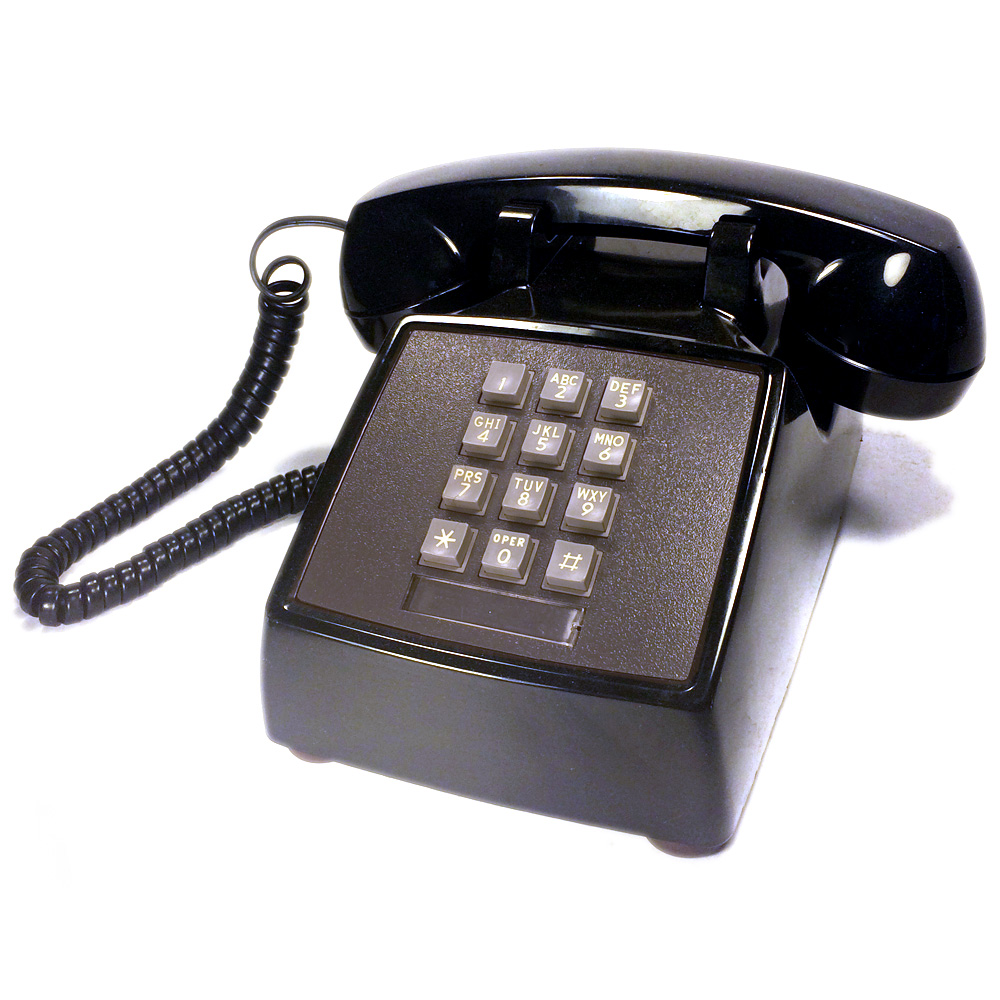
\includegraphics[width=0.6\linewidth]{img/phone_wiki.jpg}
%\footnote{\url{https://upload.wikimedia.org/wikipedia/commons/8/81/AT%26T_push_button_telephone_western_electric_model_2500_dmg_black.jpg}}
\end{frame}

\begin{frame}{An analog dial pad}
\centering
\begin{tabular}{c c c c}
      & 1209 Hz & 1336 Hz & 1477 Hz \\
697 Hz   & \textcolor{red}{1}    & 2       & 3    \\  
770 Hz   & 4    & \textcolor{red}{5}       & 6    \\
852 Hz   & 7    & 8       & \textcolor{red}{9}    \\
941 Hz   & *    & 0       & \#     \\
\end{tabular}

\begin{center}
\href{run:./phone_seq.wav}{dial}
\end{center}
\end{frame}


\begin{frame}{The time domain signal}
\centering
\begin{figure}
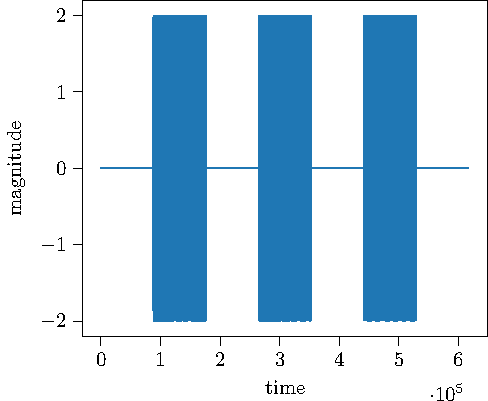
\includegraphics[width=.6\linewidth]{plots/seq_plot.pdf}
\caption{The time domain signal sampled at 44.1khz}
\end{figure}
\end{frame}

\begin{frame}{The Fourier Transform}
Forward:
\begin{equation}
% \bX_m(\omega, Sm) 
   \mathbf{X}(\omega) = \mathcal{F}\left(\mathbf{x}\right) = \sum_{t = -\infty}^{\infty} \mathbf{x}[t]e^{-j\omega t},
    \label{eq:STFT}
\end{equation}
Euler's formula:
\begin{equation}
e^{j\omega} = \cos(\omega) + j\sin (\omega)
\end{equation}
Backward:
\begin{equation}
% \bX_m(\omega, Sm) 
   \mathbf{x}(t) = \mathcal{F}^{-1}\left(\mathbf{X}\right) = \sum_{\omega = -\infty}^{\infty} \mathbf{X}[\omega]e^{j \omega t},
    \label{eq:STFT}
\end{equation}
\end{frame}


\begin{frame}{The Fourier-transfrom applied}
\centering
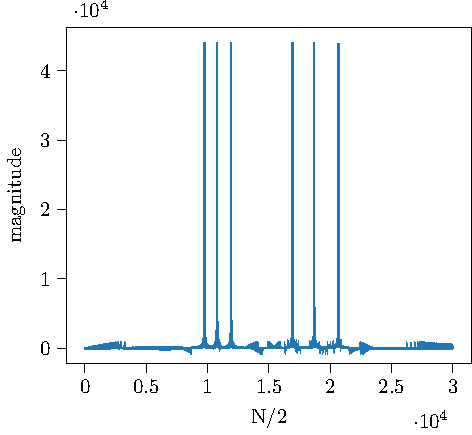
\includegraphics[width=.6\linewidth]{plots/fft.pdf}
\end{frame}


\begin{frame}{The Short time Fourier transform}
\begin{equation}
    % \bX_m(\omega, Sm) 
    \mathbf{X} [\omega, Sm] 
    = \mathcal{F}_s\left(\mathbf{x}\right) = \mathcal{F}\left(\mathbf{w}[Sm - l]\mathbf{x}[l]\right) = \sum_{l = -\infty}^{\infty} \mathbf{w}[Sm - l]\mathbf{x}[l]e^{-j\omega l},
    \label{eq:STFT}
\end{equation}
\begin{figure}
    \centering
    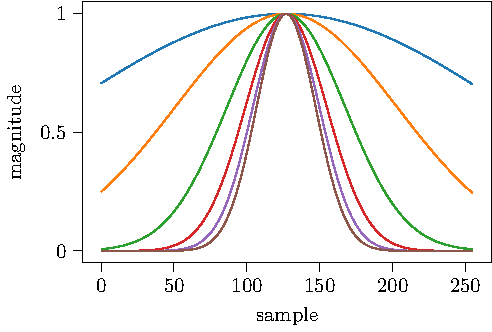
\includegraphics[width=0.49\linewidth]{./img/gaussian_window_sigma_plot.pdf}
    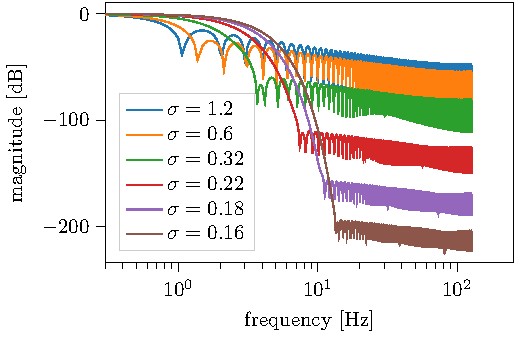
\includegraphics[width=0.49\linewidth]{./img/gaussian_window_sigma_freq_plot.pdf}
\end{figure}
\end{frame}

\begin{frame}{Short Time Fourier Transform Magnitude}
\centering
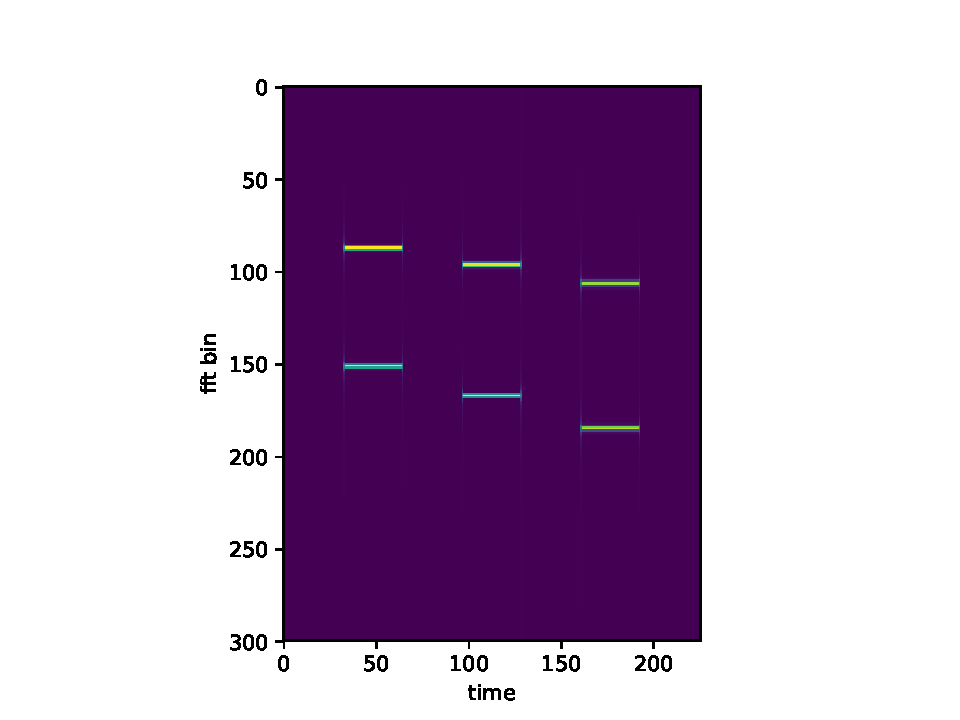
\includegraphics[width=0.8\linewidth]{./plots/stft_full.pdf}
\end{frame}

\begin{frame}{Key 1}
\centering
\begin{figure}
\scalebox{0.5}{%
\begin{tabular}{c c c c}
      & 1209 Hz & 1336 Hz & 1477 Hz \\
697 Hz   & \textcolor{red}{1}    & 2       & 3    \\  
770 Hz   & 4    & \textcolor{red}{5}       & 6    \\
852 Hz   & 7    & 8       & \textcolor{red}{9}    \\
941 Hz   & *    & 0       & \#     \\
\end{tabular}}
\end{figure}
\begin{figure}
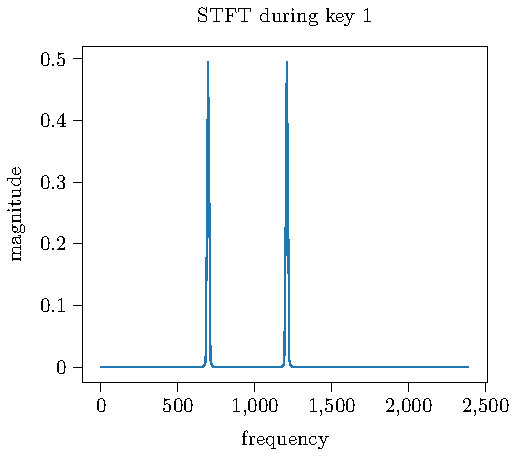
\includegraphics[width=0.45\linewidth]{./plots/stft_key_1.pdf}
\end{figure}
\end{frame}

\begin{frame}{Key 2}
\centering
\begin{figure}
\scalebox{0.5}{%
\begin{tabular}{c c c c}
      & 1209 Hz & 1336 Hz & 1477 Hz \\
697 Hz   & \textcolor{red}{1}    & 2       & 3    \\  
770 Hz   & 4    & \textcolor{red}{5}       & 6    \\
852 Hz   & 7    & 8       & \textcolor{red}{9}    \\
941 Hz   & *    & 0       & \#     \\
\end{tabular}}
\end{figure}
\begin{figure}
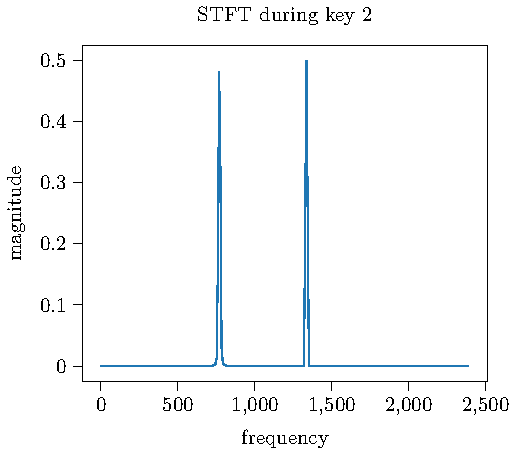
\includegraphics[width=0.5\linewidth]{./plots/stft_key_2.pdf}
\end{figure}
\end{frame}

\begin{frame}{Key 3}
\centering
\begin{figure}
\scalebox{0.5}{%
\begin{tabular}{c c c c}
      & 1209 Hz & 1336 Hz & 1477 Hz \\
697 Hz   & \textcolor{red}{1}    & 2       & 3    \\  
770 Hz   & 4    & \textcolor{red}{5}       & 6    \\
852 Hz   & 7    & 8       & \textcolor{red}{9}    \\
941 Hz   & *    & 0       & \#     \\
\end{tabular}}
\end{figure}
\begin{figure}
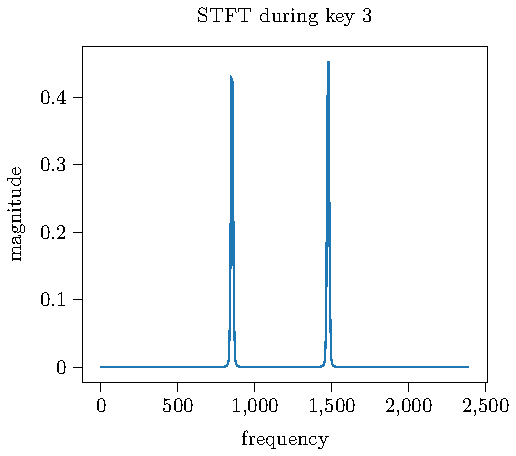
\includegraphics[width=0.5\linewidth]{./plots/stft_key_3.pdf}
\end{figure}
\end{frame}

\begin{frame}{The uncertainty principle \footnote{\url{http://newt.phys.unsw.edu.au/jw/uncertainty.html}}}
Example 1:
\begin{itemize}
\item \href{run:./sounds/heisenberg/400+403-80ms.wav}{80ms}
\item \href{run:./sounds/heisenberg/400+403-170ms.wav}{170ms}
\item \href{run:./sounds/heisenberg/400+403-330ms.wav}{330ms}
\item \href{run:./sounds/heisenberg/400+403-670ms.wav}{670ms}
\item \href{run:./sounds/heisenberg/400+403-1s.wav}{1s}
\item \href{run:./sounds/heisenberg/400+403-2s.wav}{2s}
\item \href{run:./sounds/heisenberg/400+403-5s.wav}{5s}
\end{itemize}
\end{frame}

\begin{frame}{The uncertainty principle 2\footnote{\url{http://newt.phys.unsw.edu.au/jw/uncertainty.html}}}
Example 2:
\begin{itemize}
\item \href{run:./sounds/heisenberg/400+401-80ms.wav}{80ms}
\item \href{run:./sounds/heisenberg/400+401-170ms.wav}{170ms}
\item \href{run:./sounds/heisenberg/400+401-330ms.wav}{330ms}
\item \href{run:./sounds/heisenberg/400+401-670ms.wav}{670ms}
\item \href{run:./sounds/heisenberg/400+401-1s.wav}{1s}
\item \href{run:./sounds/heisenberg/400+401-2s.wav}{2s}
\item \href{run:./sounds/heisenberg/400+401-5s.wav}{5s}
\end{itemize}
\end{frame}


\begin{frame}{Learning trough the STFT}
\begin{itemize}
\item The first example consisted a 400 and 403Hz Sine wave.
\item The second of a 400 and 401Hz Sine wave.
\item Time and frequency resolution are coupled trough the uncertainty principle.
\item Working in the time domain can overloads RNNs for long sequences.
\item Transfer a signal into the Frequency domain do the prediction and compute the inverse transform.
\item IDEA: Learn the window shape.

\end{itemize}
\end{frame}

\begin{frame}{Learning trough the STFT}
\begin{equation}
    % \bX_m(\omega, Sm) 
    \mathbf{X} [\omega, Sm] 
    = \mathcal{F}_s\left(\mathbf{x}\right) = \mathcal{F}\left(\mathbf{w}[Sm - l]\mathbf{x}[l]\right) = \sum_{l = -\infty}^{\infty} \mathbf{w}[Sm - l]\mathbf{x}[l]e^{-j\omega l},
    \label{eq:STFT}
\end{equation}
\begin{figure}
    \centering
    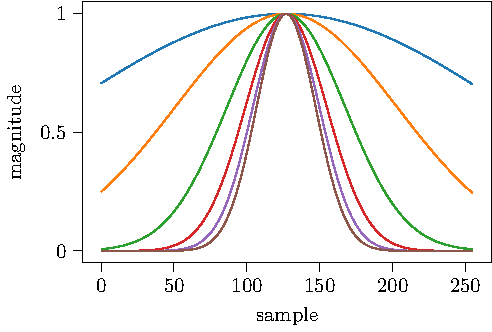
\includegraphics[width=0.49\linewidth]{./img/gaussian_window_sigma_plot.pdf}
    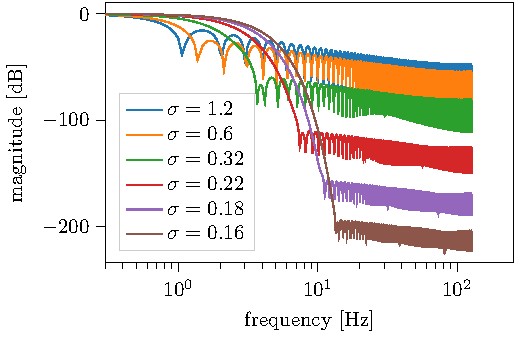
\includegraphics[width=0.49\linewidth]{./img/gaussian_window_sigma_freq_plot.pdf}
\end{figure}
\end{frame}


\begin{frame}{The European Power Grid}
\centering
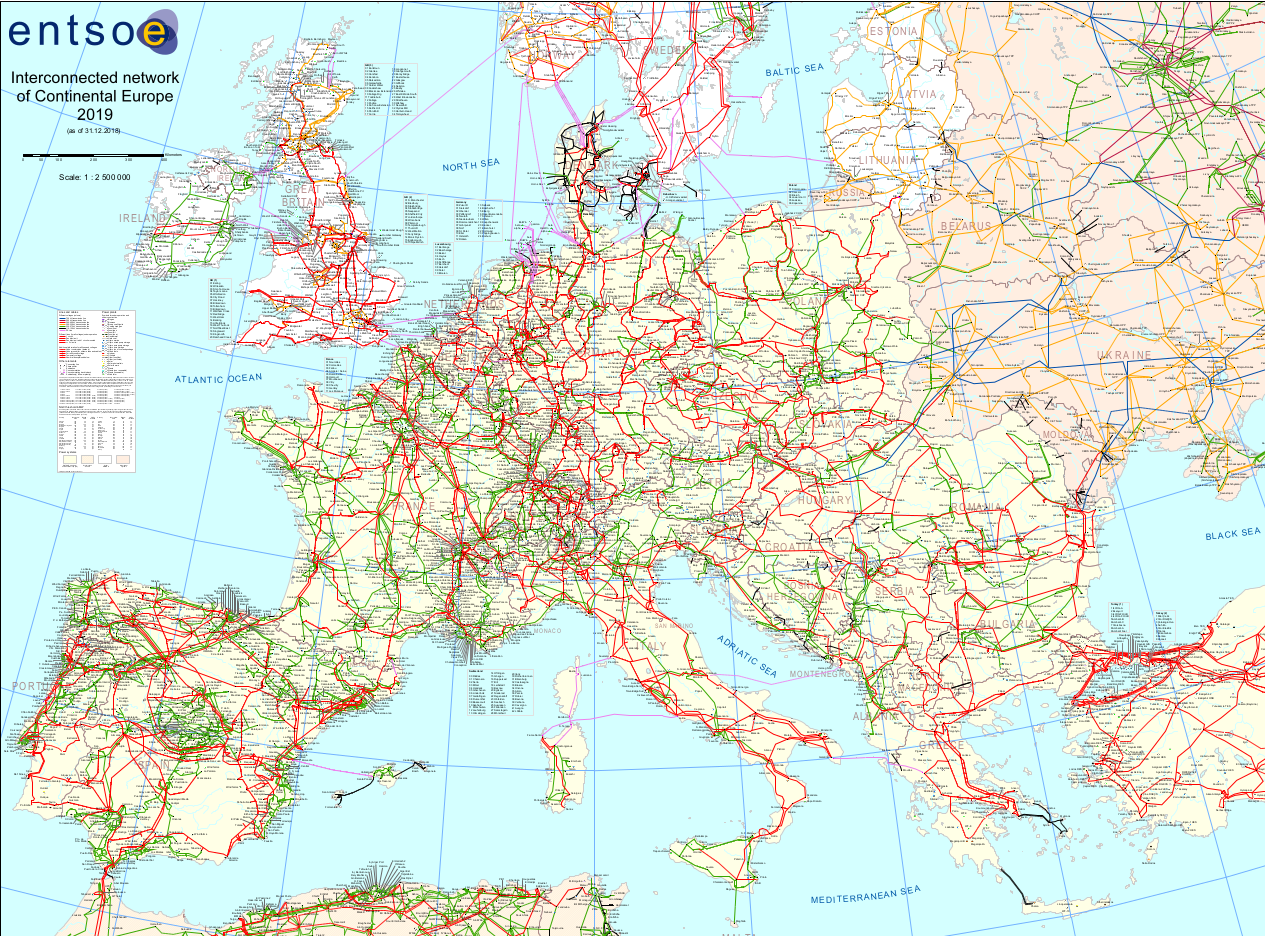
\includegraphics[width=.8\linewidth]{./img/power_grid.png}
\end{frame}

\begin{frame}{Learning trough the STFT \cite{wolter2018Fourier}}
\begin{figure}
    \centering
    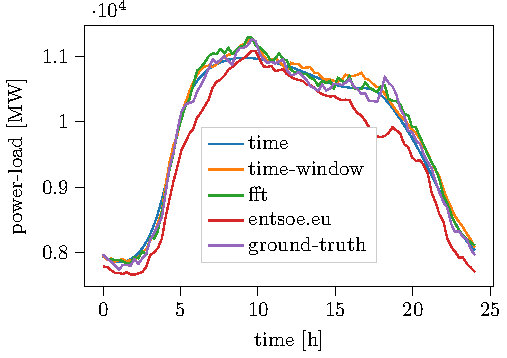
\includegraphics[width=0.49\linewidth]{./img/day_ahead_plot.pdf}
    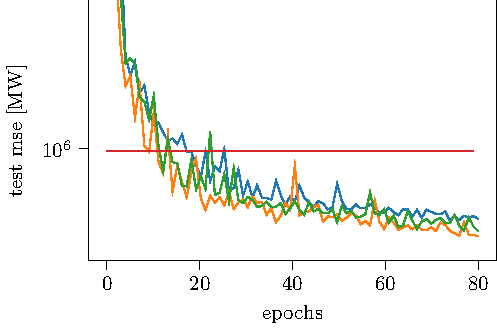
\includegraphics[width=0.49\linewidth]{./img/power_pred_15min_1d_test.pdf}
\end{figure}
\end{frame}

\begin{frame}{Learning trough the STFT \cite{wolter2018Fourier}}
\centering
\begin{tabular}{c c c c}
  Network   & mse [MW] & weights  & run [min]  \\\hline 
  time-RNN   & $1.3 \cdot 10^7$&  13k & 772 \\
  time-RNN-windowed   & $8.8 \cdot 10^5$&  28k & 12 \\
  fRNN   & $8.3 \cdot 10^5$&  44k & 13 \\
  fRNN-lowpass-1/4   & $7.6 \cdot 10^5$&  20k & 13 \\
  fRNN-lowpass-1/8   & $1.3 \cdot 10^6$&  16k & 13 \\
\end{tabular}
\begin{figure}
    \centering
    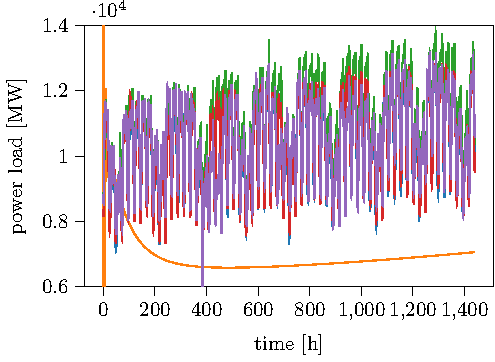
\includegraphics[width=0.48\linewidth]{./img/comparison_60d_fit.pdf}
    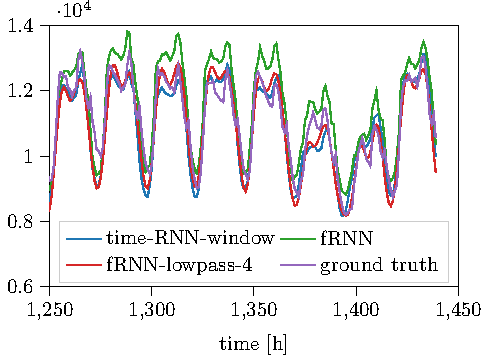
\includegraphics[width=0.48\linewidth]{./img/comparison_last_week_60d_fit.pdf}
\end{figure}
\end{frame}

\begin{frame}{Summary}
\begin{itemize}
\item The Fourier transforms finds frequency components.
\item The short time Fourier transform preserves time information.
\item Heisenberg tells us that time and frequency resolution are coupled.
\item Working in the frequency domain makes machine learning more efficient.
\item The frequency domain is complex valued and required complex networks \cite{wolter2018complexgated}.
\item Most of my work, including todays talk is free and on git-hub \url{https://github.com/v0lta}.
\end{itemize}

\end{frame}


% \begin{frame}{Complex Machine learning}
% \begin{itemize}
%   \item Quantum computers require complex unitary weights.
%   \item Fourier transforms produce complex representations.
%   \item Encoding data in magnitude and phase may enable us create a richer representation.
%   \item Complex analysis is a well studied (and very interesting!) subject,
%         lets merge it with machine learning and see what happens.
% \end{itemize}
% \end{frame}

% \begin{frame}{Memory and adding benchmark problems for RNNs}

% \begin{figure}
%   \begingroup
%   \tikzset{every picture/.style={scale=0.8}}%
%   % This file was created by matplotlib2tikz v0.6.18.
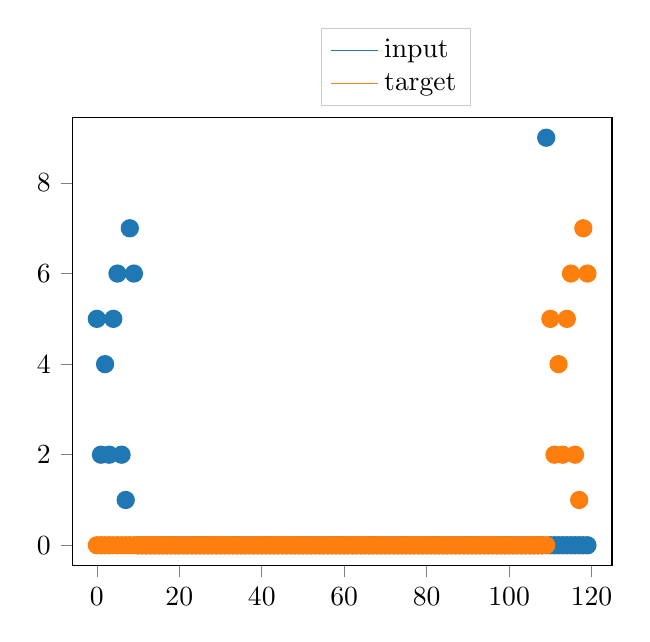
\begin{tikzpicture}

\definecolor{color0}{rgb}{0.12156862745098,0.466666666666667,0.705882352941177}
\definecolor{color1}{rgb}{1,0.498039215686275,0.0549019607843137}

\begin{axis}[
legend cell align={left},
legend entries={{input},{target}},
legend style={at={(0.6,1.2)}, anchor=north, draw=white!80.0!black},
tick align=outside,
tick pos=left,
x grid style={white!69.01960784313725!black},
xmin=-5.95, xmax=124.95,
y grid style={white!69.01960784313725!black},
ymin=-0.45, ymax=9.45
]
\addlegendimage{no markers, color0}
\addlegendimage{no markers, color1}
\addplot [semithick, color0, mark=*, mark size=3, mark options={solid}, only marks]
table [row sep=\\]{%
0	5 \\
1	2 \\
2	4 \\
3	2 \\
4	5 \\
5	6 \\
6	2 \\
7	1 \\
8	7 \\
9	6 \\
10	0 \\
11	0 \\
12	0 \\
13	0 \\
14	0 \\
15	0 \\
16	0 \\
17	0 \\
18	0 \\
19	0 \\
20	0 \\
21	0 \\
22	0 \\
23	0 \\
24	0 \\
25	0 \\
26	0 \\
27	0 \\
28	0 \\
29	0 \\
30	0 \\
31	0 \\
32	0 \\
33	0 \\
34	0 \\
35	0 \\
36	0 \\
37	0 \\
38	0 \\
39	0 \\
40	0 \\
41	0 \\
42	0 \\
43	0 \\
44	0 \\
45	0 \\
46	0 \\
47	0 \\
48	0 \\
49	0 \\
50	0 \\
51	0 \\
52	0 \\
53	0 \\
54	0 \\
55	0 \\
56	0 \\
57	0 \\
58	0 \\
59	0 \\
60	0 \\
61	0 \\
62	0 \\
63	0 \\
64	0 \\
65	0 \\
66	0 \\
67	0 \\
68	0 \\
69	0 \\
70	0 \\
71	0 \\
72	0 \\
73	0 \\
74	0 \\
75	0 \\
76	0 \\
77	0 \\
78	0 \\
79	0 \\
80	0 \\
81	0 \\
82	0 \\
83	0 \\
84	0 \\
85	0 \\
86	0 \\
87	0 \\
88	0 \\
89	0 \\
90	0 \\
91	0 \\
92	0 \\
93	0 \\
94	0 \\
95	0 \\
96	0 \\
97	0 \\
98	0 \\
99	0 \\
100	0 \\
101	0 \\
102	0 \\
103	0 \\
104	0 \\
105	0 \\
106	0 \\
107	0 \\
108	0 \\
109	9 \\
110	0 \\
111	0 \\
112	0 \\
113	0 \\
114	0 \\
115	0 \\
116	0 \\
117	0 \\
118	0 \\
119	0 \\
};
\addplot [semithick, color1, mark=*, mark size=3, mark options={solid}, only marks]
table [row sep=\\]{%
0	0 \\
1	0 \\
2	0 \\
3	0 \\
4	0 \\
5	0 \\
6	0 \\
7	0 \\
8	0 \\
9	0 \\
10	0 \\
11	0 \\
12	0 \\
13	0 \\
14	0 \\
15	0 \\
16	0 \\
17	0 \\
18	0 \\
19	0 \\
20	0 \\
21	0 \\
22	0 \\
23	0 \\
24	0 \\
25	0 \\
26	0 \\
27	0 \\
28	0 \\
29	0 \\
30	0 \\
31	0 \\
32	0 \\
33	0 \\
34	0 \\
35	0 \\
36	0 \\
37	0 \\
38	0 \\
39	0 \\
40	0 \\
41	0 \\
42	0 \\
43	0 \\
44	0 \\
45	0 \\
46	0 \\
47	0 \\
48	0 \\
49	0 \\
50	0 \\
51	0 \\
52	0 \\
53	0 \\
54	0 \\
55	0 \\
56	0 \\
57	0 \\
58	0 \\
59	0 \\
60	0 \\
61	0 \\
62	0 \\
63	0 \\
64	0 \\
65	0 \\
66	0 \\
67	0 \\
68	0 \\
69	0 \\
70	0 \\
71	0 \\
72	0 \\
73	0 \\
74	0 \\
75	0 \\
76	0 \\
77	0 \\
78	0 \\
79	0 \\
80	0 \\
81	0 \\
82	0 \\
83	0 \\
84	0 \\
85	0 \\
86	0 \\
87	0 \\
88	0 \\
89	0 \\
90	0 \\
91	0 \\
92	0 \\
93	0 \\
94	0 \\
95	0 \\
96	0 \\
97	0 \\
98	0 \\
99	0 \\
100	0 \\
101	0 \\
102	0 \\
103	0 \\
104	0 \\
105	0 \\
106	0 \\
107	0 \\
108	0 \\
109	0 \\
110	5 \\
111	2 \\
112	4 \\
113	2 \\
114	5 \\
115	6 \\
116	2 \\
117	1 \\
118	7 \\
119	6 \\
};
\end{axis}

\end{tikzpicture}
%   % This file was created by matplotlib2tikz v0.6.18.
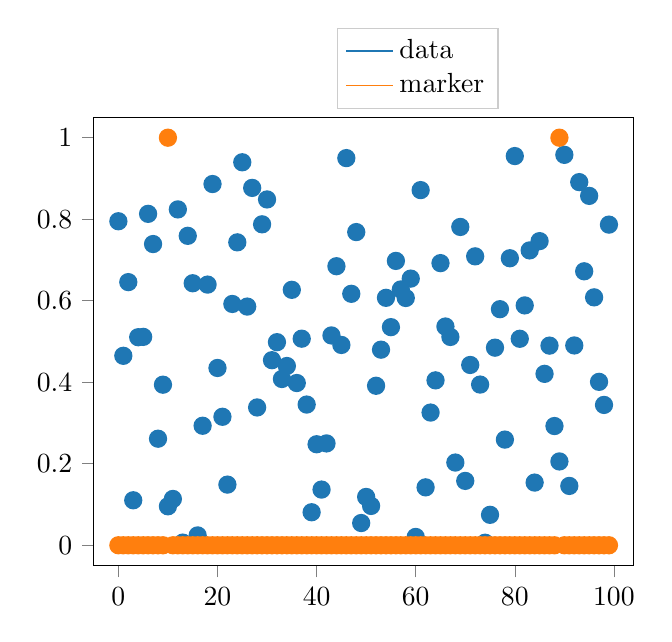
\begin{tikzpicture}

\definecolor{color0}{rgb}{0.12156862745098,0.466666666666667,0.705882352941177}
\definecolor{color1}{rgb}{1,0.498039215686275,0.0549019607843137}

\begin{axis}[
legend cell align={left},
legend entries={{data},{marker}},
legend style={at={(0.6,1.2)}, anchor=north, draw=white!80.0!black},
tick align=outside,
tick pos=left,
x grid style={white!69.01960784313725!black},
xmin=-4.95, xmax=103.95,
y grid style={white!69.01960784313725!black},
ymin=-0.05, ymax=1.05
]
\addlegendimage{no markers, color0}
\addlegendimage{no markers, color1}
\addplot [semithick, color0, mark=*, mark size=3, mark options={solid}, only marks]
table [row sep=\\]{%
0	0.795019845599018 \\
1	0.464894663895327 \\
2	0.645689818059632 \\
3	0.110404376572817 \\
4	0.510464880117213 \\
5	0.511325199051234 \\
6	0.813155032858877 \\
7	0.739088424364177 \\
8	0.261479380793186 \\
9	0.393983581646967 \\
10	0.0955843557375171 \\
11	0.11362414465094 \\
12	0.824064830816347 \\
13	0.00653479542503921 \\
14	0.759220491228536 \\
15	0.642901767181444 \\
16	0.0241655803486288 \\
17	0.293228995729676 \\
18	0.639586373261765 \\
19	0.886351458119477 \\
20	0.435026013531375 \\
21	0.315274664774964 \\
22	0.148813841534109 \\
23	0.592055702306838 \\
24	0.743274638757777 \\
25	0.939698460197675 \\
26	0.585622712337468 \\
27	0.87686485422555 \\
28	0.338135208208416 \\
29	0.787487145108367 \\
30	0.848528041904568 \\
31	0.45409598693934 \\
32	0.498318768598199 \\
33	0.407943671885351 \\
34	0.43987060441292 \\
35	0.626769749050435 \\
36	0.398114642470146 \\
37	0.506851755820912 \\
38	0.345293988116787 \\
39	0.0810231302245875 \\
40	0.24784627543168 \\
41	0.136656861495367 \\
42	0.249851290064188 \\
43	0.51482647485681 \\
44	0.684679304659001 \\
45	0.49148677228776 \\
46	0.949977076015945 \\
47	0.616994835574287 \\
48	0.768437668632366 \\
49	0.0545989447654387 \\
50	0.118612915627734 \\
51	0.0965307905405638 \\
52	0.391365207292609 \\
53	0.47987461728131 \\
54	0.607123542749167 \\
55	0.535186740116049 \\
56	0.697775729312253 \\
57	0.627653553760089 \\
58	0.606726096275297 \\
59	0.654286893633733 \\
60	0.0204287467079927 \\
61	0.871464869316183 \\
62	0.142094871100816 \\
63	0.325618583106566 \\
64	0.404646643819146 \\
65	0.692236368277109 \\
66	0.536752455568487 \\
67	0.511101596076019 \\
68	0.202998342977949 \\
69	0.781038248370334 \\
70	0.157943108157318 \\
71	0.442417981403126 \\
72	0.708924188162759 \\
73	0.39428940019825 \\
74	0.00622192562292434 \\
75	0.0747313101021986 \\
76	0.484830634239883 \\
77	0.579262220652348 \\
78	0.259264898936668 \\
79	0.70422719363416 \\
80	0.954967802904909 \\
81	0.506623672894714 \\
82	0.588543846313598 \\
83	0.723473653845397 \\
84	0.153822997897741 \\
85	0.746229926073241 \\
86	0.42060034992435 \\
87	0.489860994364912 \\
88	0.292587178845884 \\
89	0.205666921389715 \\
90	0.957909437737243 \\
91	0.145618305065359 \\
92	0.490268452960524 \\
93	0.890993593990406 \\
94	0.672230633869469 \\
95	0.857272157280991 \\
96	0.608286150040313 \\
97	0.400982212033234 \\
98	0.344331178044672 \\
99	0.786701573711393 \\
};
\addplot [semithick, color1, mark=*, mark size=3, mark options={solid}, only marks]
table [row sep=\\]{%
0	0 \\
1	0 \\
2	0 \\
3	0 \\
4	0 \\
5	0 \\
6	0 \\
7	0 \\
8	0 \\
9	0 \\
10	1 \\
11	0 \\
12	0 \\
13	0 \\
14	0 \\
15	0 \\
16	0 \\
17	0 \\
18	0 \\
19	0 \\
20	0 \\
21	0 \\
22	0 \\
23	0 \\
24	0 \\
25	0 \\
26	0 \\
27	0 \\
28	0 \\
29	0 \\
30	0 \\
31	0 \\
32	0 \\
33	0 \\
34	0 \\
35	0 \\
36	0 \\
37	0 \\
38	0 \\
39	0 \\
40	0 \\
41	0 \\
42	0 \\
43	0 \\
44	0 \\
45	0 \\
46	0 \\
47	0 \\
48	0 \\
49	0 \\
50	0 \\
51	0 \\
52	0 \\
53	0 \\
54	0 \\
55	0 \\
56	0 \\
57	0 \\
58	0 \\
59	0 \\
60	0 \\
61	0 \\
62	0 \\
63	0 \\
64	0 \\
65	0 \\
66	0 \\
67	0 \\
68	0 \\
69	0 \\
70	0 \\
71	0 \\
72	0 \\
73	0 \\
74	0 \\
75	0 \\
76	0 \\
77	0 \\
78	0 \\
79	0 \\
80	0 \\
81	0 \\
82	0 \\
83	0 \\
84	0 \\
85	0 \\
86	0 \\
87	0 \\
88	0 \\
89	1 \\
90	0 \\
91	0 \\
92	0 \\
93	0 \\
94	0 \\
95	0 \\
96	0 \\
97	0 \\
98	0 \\
99	0 \\
};
\end{axis}

\end{tikzpicture}
%   \endgroup
%   \caption{Illustrations of the memory problem on the left and the
%            adding problem on the right.}
%   %
% \end{figure}
% \end{frame}

% \begin{frame}{Wirtinger-Calculus \cite{Wirtinger}\cite{Mandic}\cite{Delgado}}
% For a complex function $f(z) = u(x,y) - iv(x,y)$ we have:
% \begin{align}
%     \mathbb{R}\text{-derivative} \triangleq \frac{\partial f}{\partial z}|_{\bar{z}=\text{const}}\ = \frac{1}{2}(\frac{\partial f}{\partial x} - i \frac{\partial f}{\partial y}),\\ \overline{\mathbb{R}}\text{-derivative} \triangleq \frac{\partial f}{\partial \bar{z}}|_{z=\text{const}} = \frac{1}{2}(\frac{\partial f}{\partial x} + i \frac{\partial f}{\partial y}).
% \end{align}
% Based on these derivatives, one can define the chain rule for a function $g(f(z))$ as follows:
% \begin{equation}
%     \frac{\partial g(f(z))}{\partial z} = \frac{\partial g}{\partial f} \frac{\partial f}{\partial z} + \frac{\partial g}{\partial \bar{f}} \frac{\partial \bar{f}}{\partial z} \text{ where } \bar{f} = u(x,y) - iv(x,y).
% \end{equation}
% Theoretical tool to convince ourselves, that it's ok to work with equivalent real networks.
% \end{frame}

% \begin{frame}{Unitary Evolution matrix RNN-Motivation \cite{Arjovsky}\cite{Pascanu}}
%   \begin{align}
%   \mathbf{x}_t  = \mathbf{W}_{\text{rec}}f(\mathbf{x}_{t-1}) + \mathbf{W}_{\text{in}}\mathbf{u}_t + \textbf{b}.
%   \end{align}
%   \begin{align}
%   \frac{\partial \mathcal{E}}{\partial \theta} &= \sum_{1 \leq t \leq T} \frac{\mathcal{E}_t}{\partial \theta}, \\
%   \frac{\partial\mathcal{E}_t}{\partial\theta} &= \sum_{1 \leq k \leq t}( \frac{\mathcal{E}_t}{\partial \mathbf{x}_t} \frac{\partial \mathbf{x}_t}{ \mathbf{x}_k} \frac{\partial^+ \mathbf{x}_k}{\partial \theta}), \label{eq:gradsum}\\
%   \frac{\partial \mathbf{x}_t}{ \partial \mathbf{x}_k} &= \prod_{t \geq i > k} \frac{\partial \mathbf{x}_i}{ \partial \mathbf{x}_{i-1}} = \prod_{t \geq i > k} W^T_{\text{rec}} \text{diag}(f'(\mathbf{x}_{i-1})).
%   \end{align}
% \end{frame}

% \begin{frame}{Stiefel Manifold Weight Updates \cite{Wisdom}}
% \begin{align}
% \mathbf{W}_{k+1} &=  (\mathbf{I} + \frac{\lambda}{2}\mathbf{A}_k)^{-1}(\mathbf{I} - \frac{\lambda}{2}\mathbf{A}_k)\mathbf{W}_k, \\
% \text{where} % \qquad \mathbf{A} &= \mathbf{W}\frac{\partial F}{\partial \mathbf{W}}^* - \mathbf{W}^*\frac{\partial F}{\partial \mathbf{W}}
% \qquad \mathbf{A} &= \mathbf{W}\overline{\nabla_{\mathbf{w}}{F}}^T - \overline{\mathbf{W}}^T\nabla_{{\mathbf{w}}}{F}.
% \label{eq:Stiefel}
% \end{align}


% \begin{figure}
%     \centering
%     \begin{tikzpicture}
%         \def\a{2}%width of rectangle
%         \def\b{\a}%height of rectangle
%         \def\lw{0.1}
%         \draw[] (0,0) rectangle (\a,\b);
%         \foreach \x in{0,0.2,0.4,...,\a}{
%         \draw [gray,line width=\lw mm](\x,0)--(0,\x);
%         \draw [gray,line width=\lw mm](\a,\x)--(\x,\b);}
%         \foreach \x in{0.1,0.3,...,\a}{
%         \draw [black,line width=\lw mm](\x,0)--(0,\x);
%         \draw [black,line width=\lw mm](\a,\x)--(\x,\b);}
%         \draw[->] (1,-0.25) -- (1,2.25cm) node[above] {$y$};
%         \draw[->] (-0.25,1) -- (2.25cm,1) node[right] {$x$};
%         \draw (2.55cm,1cm) node[above=1pt] {$(\infty,0)$};
%         \draw (1.65cm,2.05cm) node[above=1pt] {$(0,\infty)$};
%         \draw[->,thick]  (3.15cm,1) -- (3.85cm,1);
%     \end{tikzpicture}
%     \begin{tikzpicture}
%         \draw[thick] (0cm, 0cm) circle(1cm);
%         \draw[->] (0,-1.25cm) -- (0,1.25cm) node[above] {$y$};
%         \draw[->] (-1.25,0) -- (1.25cm,0) node[right] {$x$};
%         \filldraw[black] (1cm, 0) circle(1.4pt);
%         \draw (1.35cm,0cm) node[above=1pt] {$(1,0)$};
%     \end{tikzpicture}
%     \caption{Fix the optimized matrix eigenvalues onto the unit circle. The key idea behind stiefel-manifold optimization. }
% \end{figure}
% \end{frame}

% \begin{frame}{The linear unitary case}
%   \begin{align}
%   \mathbf{x}_t  = \mathbf{W}_{\text{rec}}\mathbf{x}_{t-1} + \mathbf{W}_{\text{in}}\mathbf{u}_t + \textbf{b}.
%   \end{align}
%   \begin{figure}
%     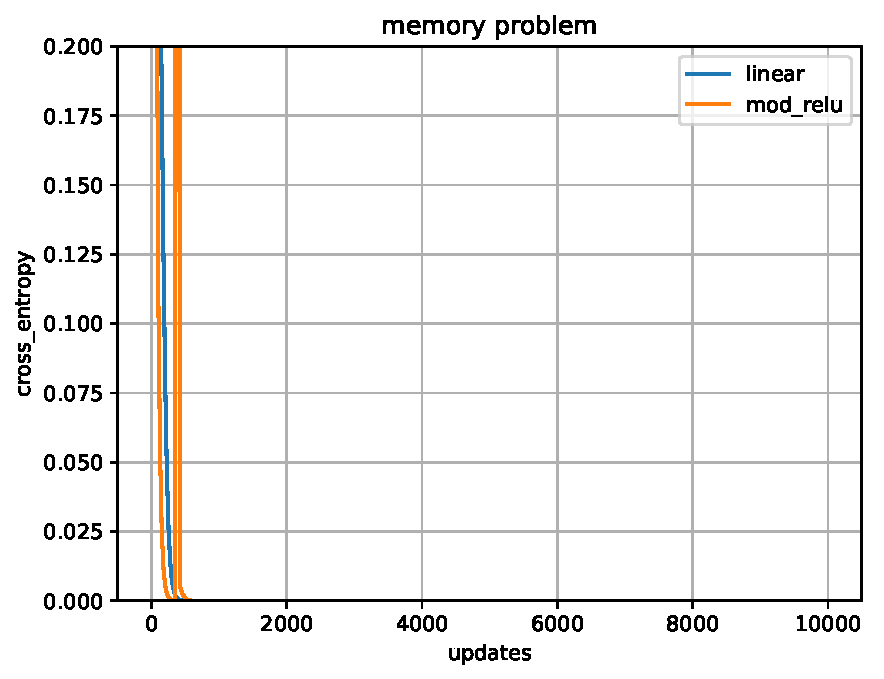
\includegraphics[width=0.4\linewidth]{img/memory_50.pdf}
%     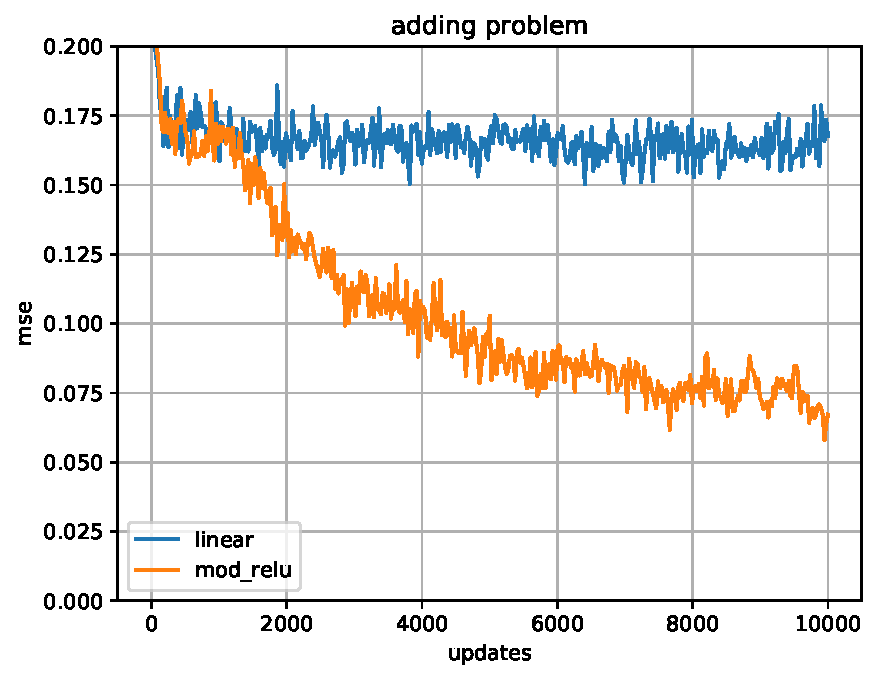
\includegraphics[width=0.4\linewidth]{img/adding_50.pdf}
%     \caption{Performance of linear and mod-Relu activated unitary RNNs on the 
%              memory (left) and adding (right) problems for T=50. All networks have
%              approx. 40k weights.}
%   \end{figure}

% \end{frame}


% \begin{frame}{Complex equivalents of $\tanh$ and Relu}
% \begin{figure}
% 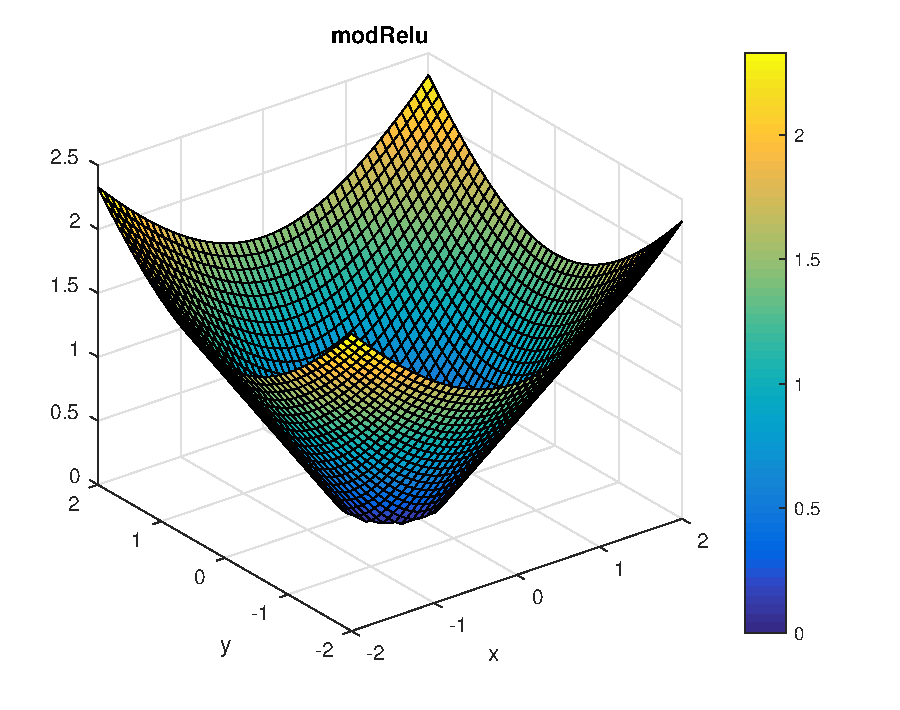
\includegraphics[width=0.4\textwidth]{img/modRelu_slice.pdf}
% 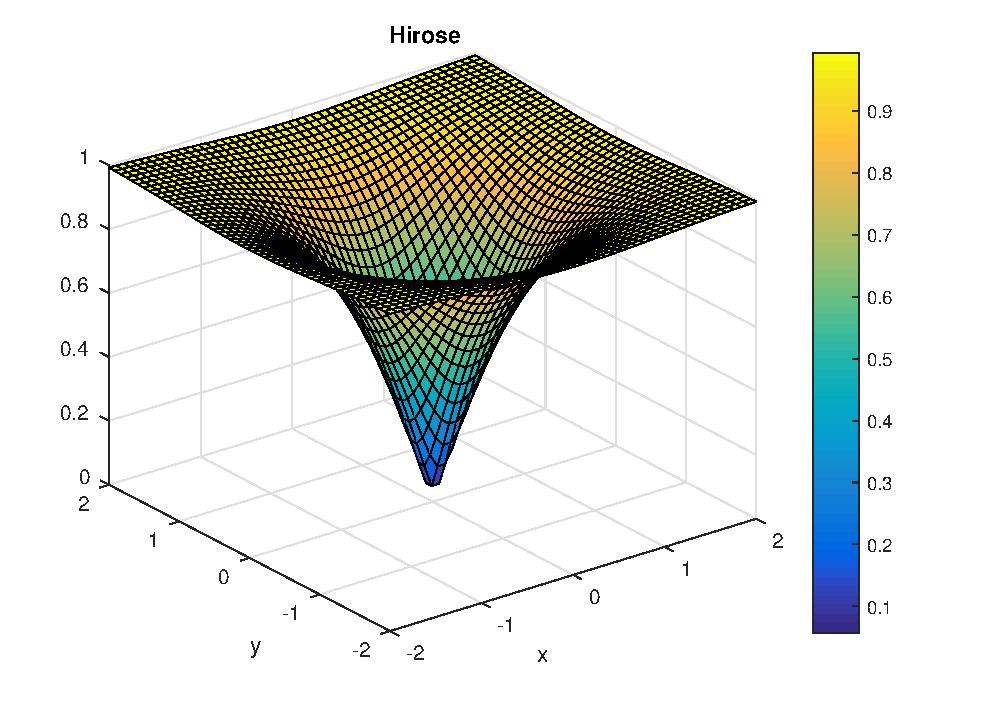
\includegraphics[width=0.4\textwidth]{img/Hirose_slice.pdf}
% \end{figure}

% \begin{equation}~\label{eq:Hirose}
%     f_{\text{Hirose}}(z) = \tanh\left(\frac{|z|}{m^2}\right)e^{-i \cdot \theta_z} = \tanh\left(\frac{|z|}{m^2}\right)\frac{z}{|z|},
% \end{equation}
% \begin{equation}~\label{eq:modrelu}
%     f_{\text{modReLU}}(z) = \text{ReLU}(|z| + b)e^{-i \cdot \theta_z} = \text{ReLU}(|z| + b)\frac{z}{|z|}.
% \end{equation}
% We will compare their performance as state-to-state non-linearities.
% \end{frame}


% \begin{frame}{Unitary evolution network performance}
% \begin{align}
%   \mathbf{x}_t  = \mathbf{U}_{\text{rec}}f(\mathbf{x}_{t-1}) + \mathbf{W}_{\text{in}}\mathbf{u}_t + \textbf{b}.
%   \end{align}
% \begin{figure}
% 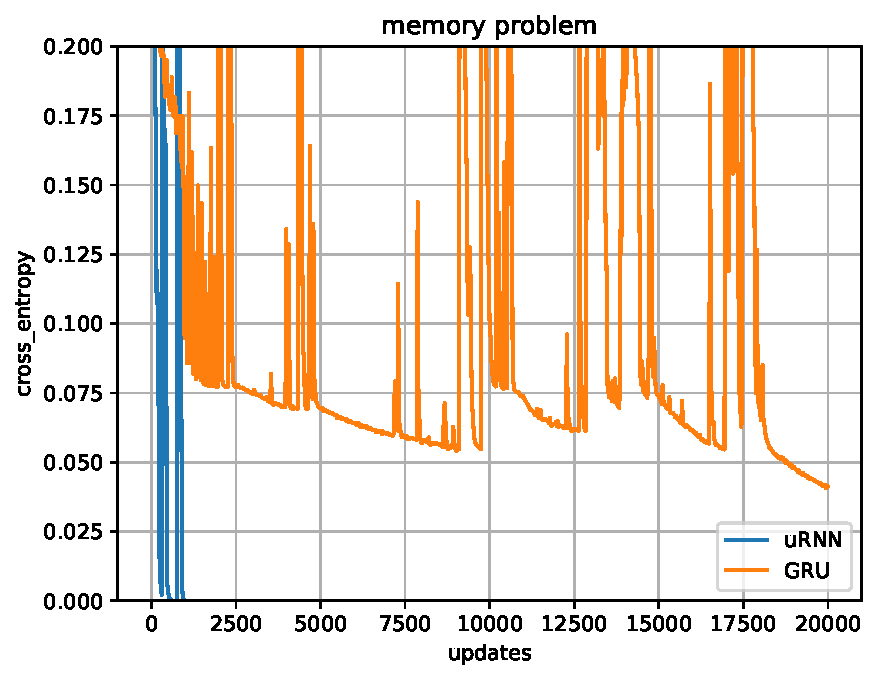
\includegraphics[width=0.4\linewidth]{img/sem_GRU_UNN_memory.pdf}
% 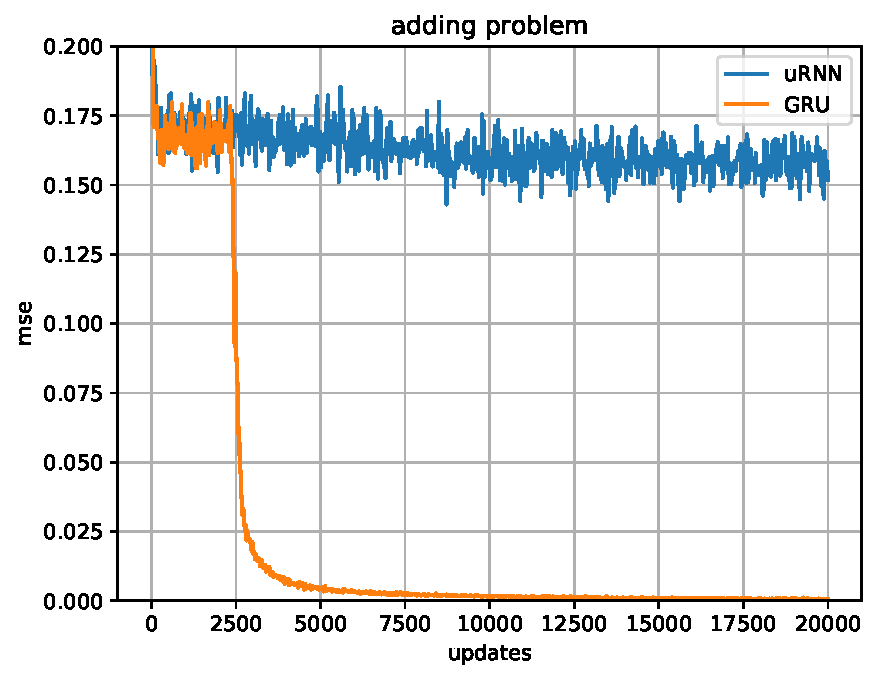
\includegraphics[width=0.4\linewidth]{img/sem_GRU_UNN_adding.pdf}
% \caption{Current state of the art performance on memory and adding problem for T=250. Models have approximately 40k weights.}
% \end{figure}
% \end{frame}

% \begin{frame}{The gated recurrent unit}
% \begin{figure}
% 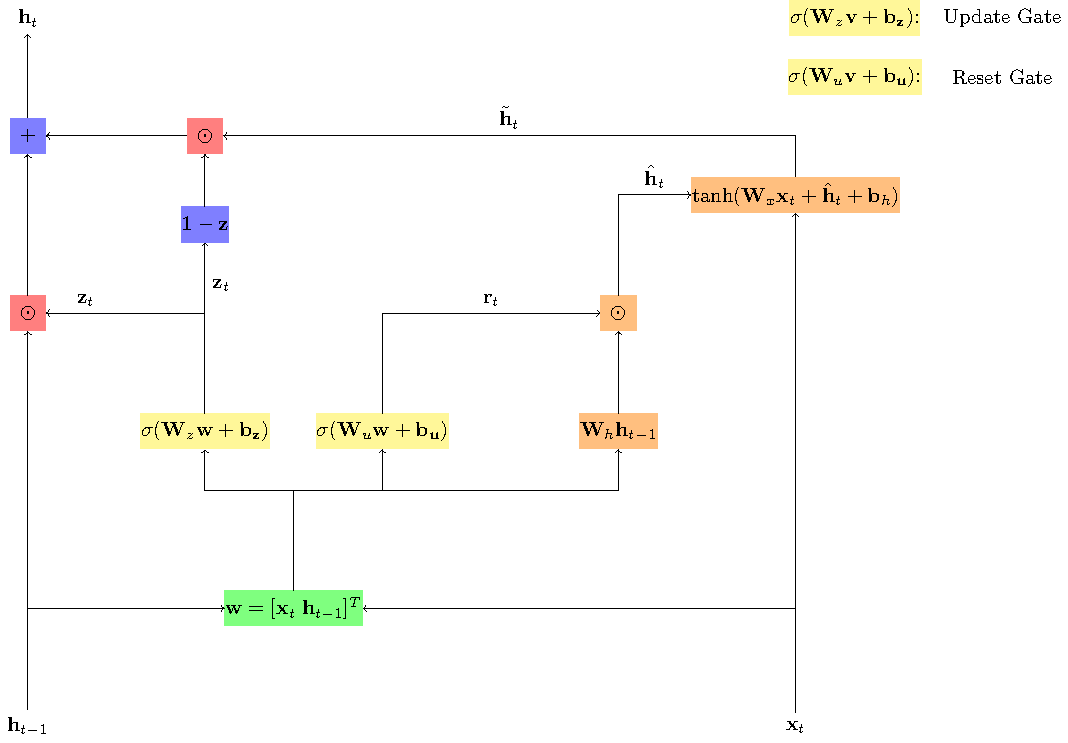
\includegraphics[width=0.88\linewidth]{img/gru.pdf}
% \end{figure}
% \end{frame}


% \begin{frame}{Complex gated Recurrent Recurrent Nets \cite{wolter2018complexgated}}
% Gate equation:
% \begin{align}
%     \mathbf{g}_r = f_g(\mathbf{z}_r), \qquad \text{where} \qquad \mathbf{z}_r 
%     = \mathbf{W}_r \mathbf{h} + \mathbf{V}_r \mathbf{x}_t + \mathbf{b}_r ,\\
%     \mathbf{g}_z = f_g(\mathbf{z}_z), \qquad \text{where} \qquad \mathbf{z}_z 
%     = \mathbf{W}_z \mathbf{h} + \mathbf{V}_z \mathbf{x}_t + \mathbf{b}_z,
%     \label{eq:dual_gate2}
% \end{align}
% Update equations:
% \begin{align}
%     \widetilde{\mathbf{z}}_{t} &= \mathbf{W} (\mathbf{g}_r \odot \mathbf{h}_{t-1}) + \mathbf{V} \mathbf{x}_{t} + \mathbf{b} \label{eq:state_candidate}, \\
%     \mathbf{h}_{t} &= \mathbf{g}_z \odot f_a(\widetilde{\mathbf{z}}_t) +(1 - \mathbf{g}_z) \odot \mathbf{h}_{t-1}, \label{eq:state_update}
% \end{align}
% $\mathbb{C} \rightarrow \mathbb{R}$, mapping:
% \begin{equation}
% \mathbf{o}_r = \mathbf{W}_o [\Re(\mathbf{h}) \; \Im(\mathbf{h})] + \mathbf{b}_o.
% \end{equation}
% \end{frame}

% \begin{frame}{Complex gate activations}
% \begin{align}
%     f_{\text{ mod sigmoid}}(\mathbf{z}) &= \sigma(\alpha \Re{(\mathbf{z})} + \beta \Im{(\mathbf{z})}).
% \end{align}
% With $\alpha \in [0,1] \text{ and } \beta = (1 - \alpha)$. \\
% \end{frame}


% \begin{frame}{Comparison to state of the art}
%   \begin{figure}
%   %\centering
%   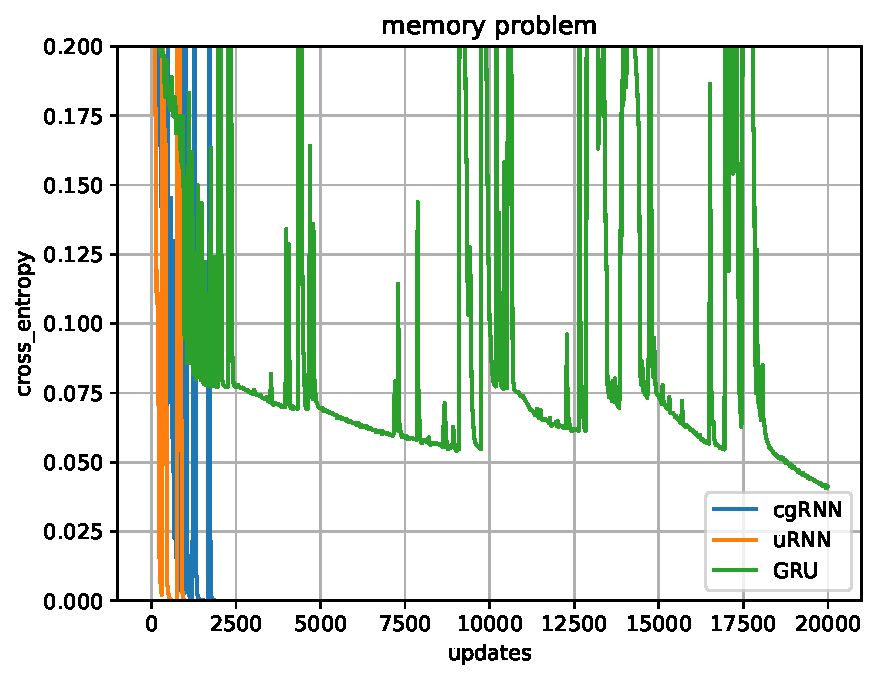
\includegraphics[width=0.4\linewidth]{./img/aaai_GRU_UNN_cgRNN_memory.pdf}
%   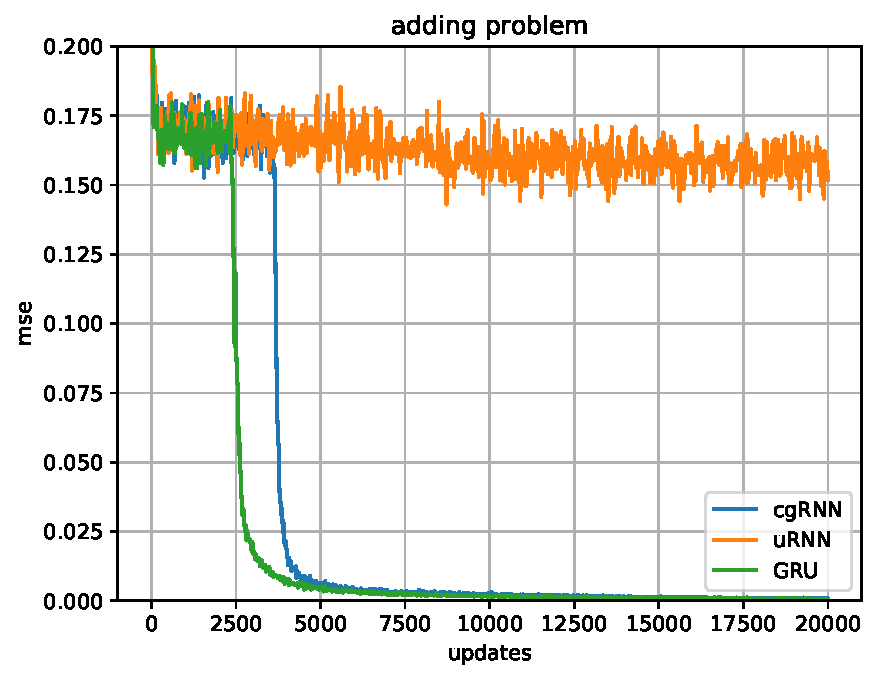
\includegraphics[width=0.4\linewidth]{./img/aaai_GRU_UNN_cgRNN_adding.pdf}%
%   \caption{\small Comparison of our complex gated RNN (cgRNN, blue, $n_h\!=\!80$) with the unitary RNN~\cite{Arjovsky}(uRNN, orange, $n_h\!=\!140$) and standard GRU~\cite{cho-al-emnlp14}(orange, $n_h\!=\!112$) on the memory (left) and adding (right) problem for $T\!=\!250$.}
%   %\label{fig:unnGRU}
%   \end{figure}
% \end{frame}

% \begin{frame}{Stiefel optimization and activations}
% \begin{figure}
%   \centering
%   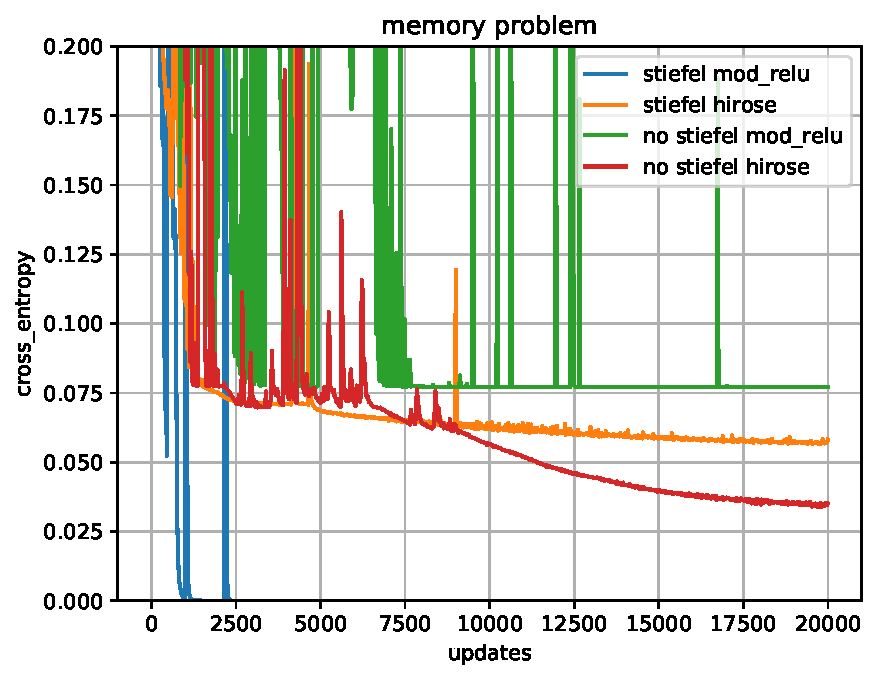
\includegraphics[width=0.4\linewidth]{./img/aaai_stiefel_bounded_memory.pdf}
%   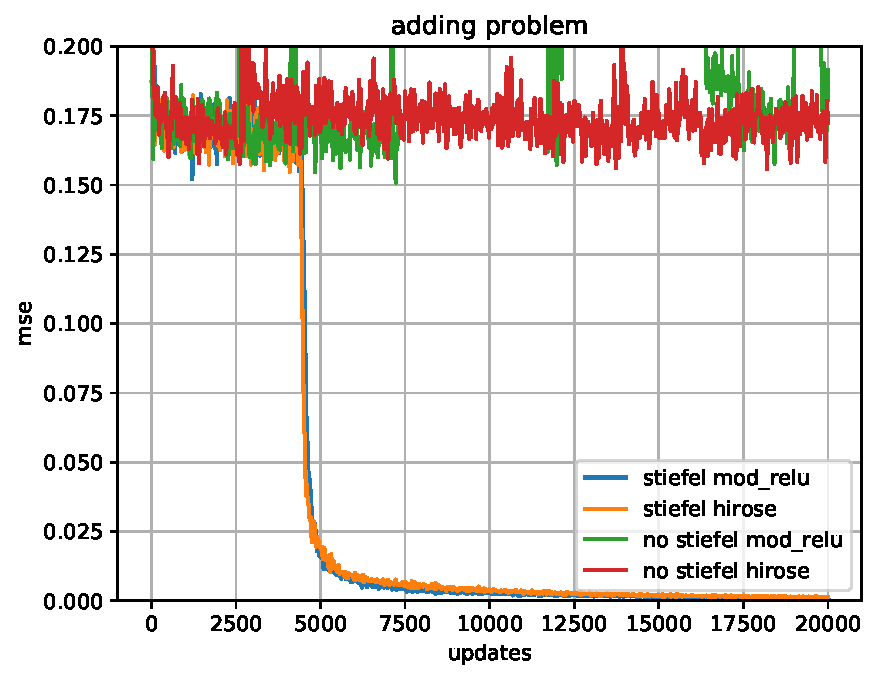
\includegraphics[width=0.4\linewidth]{./img/aaai_stiefel_bounded_adding.pdf}%
%   \caption{\small Comparison of non-linearities and norm preserving state transition matrices on the complex gated RNNs for the memory (a) and adding (b) problems for T=250. We use $n_h=80$ for all experiments.}
%   \label{fig:complex_results}
% \end{figure}
% \end{frame}

% \begin{frame}{Weight reducitons on mocap data}
% 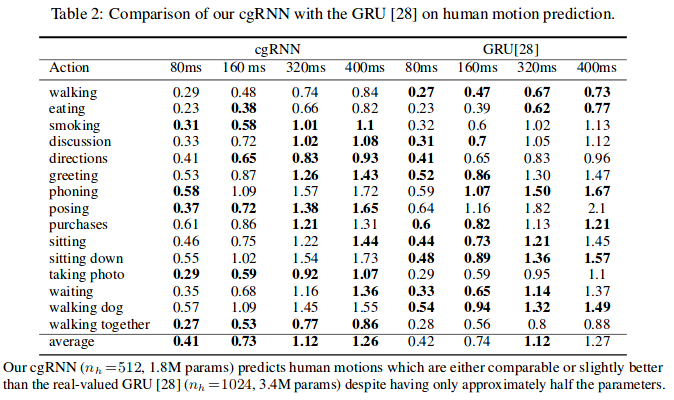
\includegraphics[scale=.4]{./img/results_paper.png}
% \end{frame}

% \begin{frame}{Upcoming: Temporal Convolutions in the frequency domain}
% \begin{itemize}
% \item The STFT turns sequences of numbers into images.
% \item What happens if we convolve these in time and frequency?
% \item What is the best way to convolve in frequency and time?
% \item How can recurrent connections and convolutions best be used together?
% \end{itemize}
% \end{frame}

\begin{frame}[allowframebreaks]
        \frametitle{References}
        \bibliographystyle{amsalpha}
        \bibliography{literature.bib}
\end{frame}


\begin{frame}{Discussion}
Thanks for your attention and feedback. \\
Feel free to contact me at: wolter@cs.uni-bonn.de
\end{frame}

\end{document}

